\smallframetitle

\section{From 17/06/24 to 21/06/24}
\insertsectionframe

\subsection{Road detection method - in progress}
\insertsubsectionframe

\begin{frame}{Methodology}
    We have seen that one classification with either DBScan or HDBScan isn't enough. So, why not combining them.
    \begin{block}{The base idea}
        We will combine the clusters of DBScan, HDBScan and OPTICS (another density base clustering method) to try to find roads.
    \end{block}

    \begin{block}{One problem}
        We are now able to detect road/railways but the problem is that there is still little clusters that are useless.
    \end{block}
\end{frame}

\begin{frame}{DBScan clustering}
    \begin{figure}
        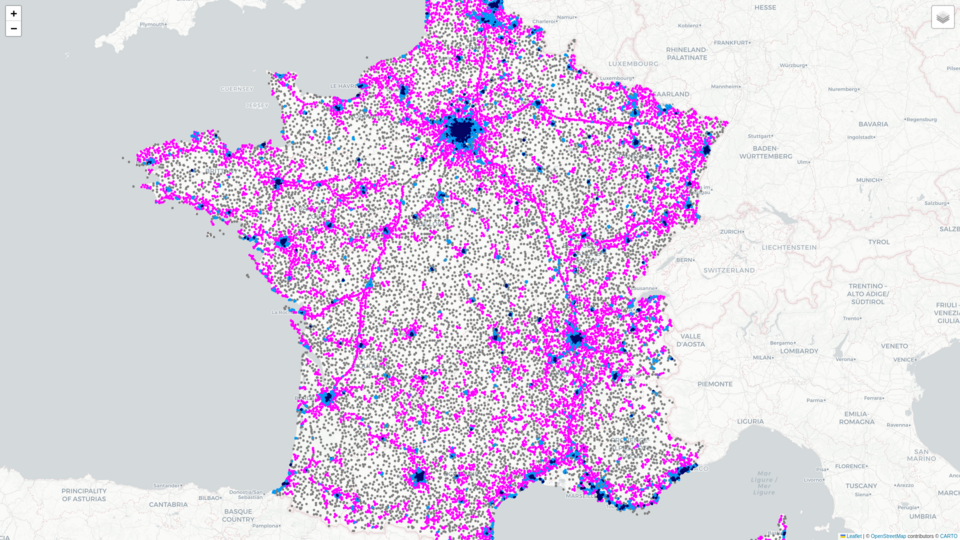
\includegraphics[height=0.6\paperheight]{images/cartes/road_detection/dbs.png}
        \caption{DBScan clustering}
    \end{figure}
\end{frame}

\begin{frame}{HDBScan clustering}
    \begin{figure}
        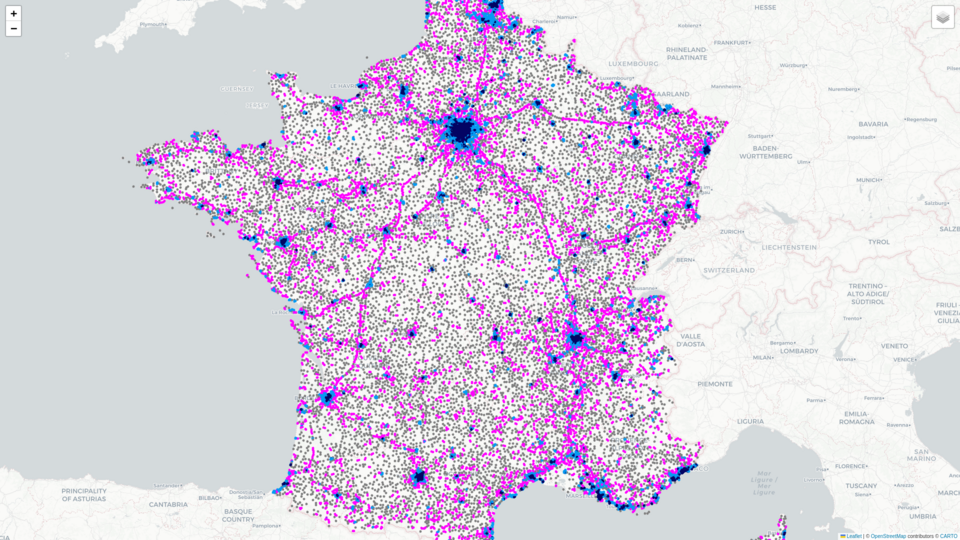
\includegraphics[height=0.6\paperheight]{images/cartes/road_detection/hdb.png}
        \caption{HDBScan clustering}
    \end{figure}
\end{frame}

\begin{frame}{OPTICS clustering}
    \begin{figure}
        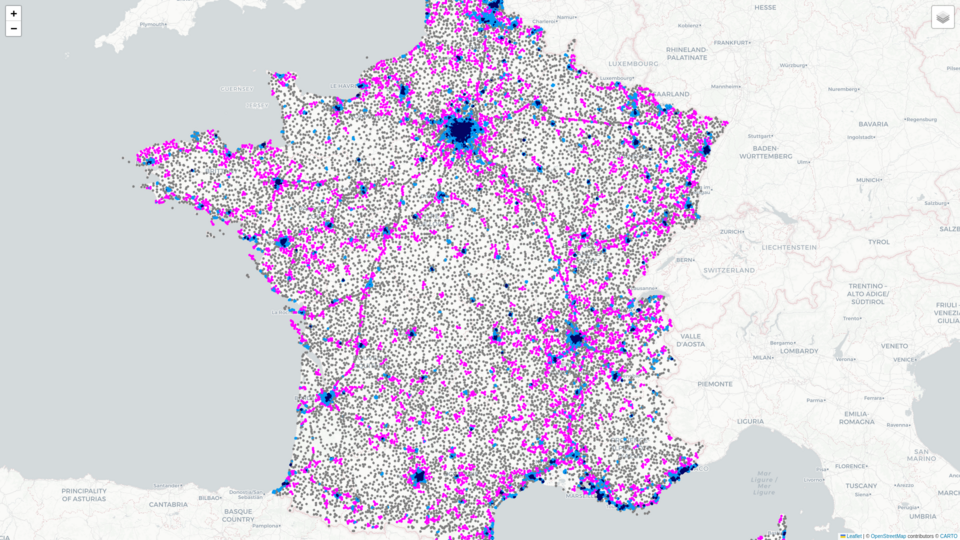
\includegraphics[height=0.6\paperheight]{images/cartes/road_detection/opt.png}
        \caption{OPTICS clustering}
    \end{figure}
\end{frame}

\begin{frame}{Result}
    \begin{figure}
        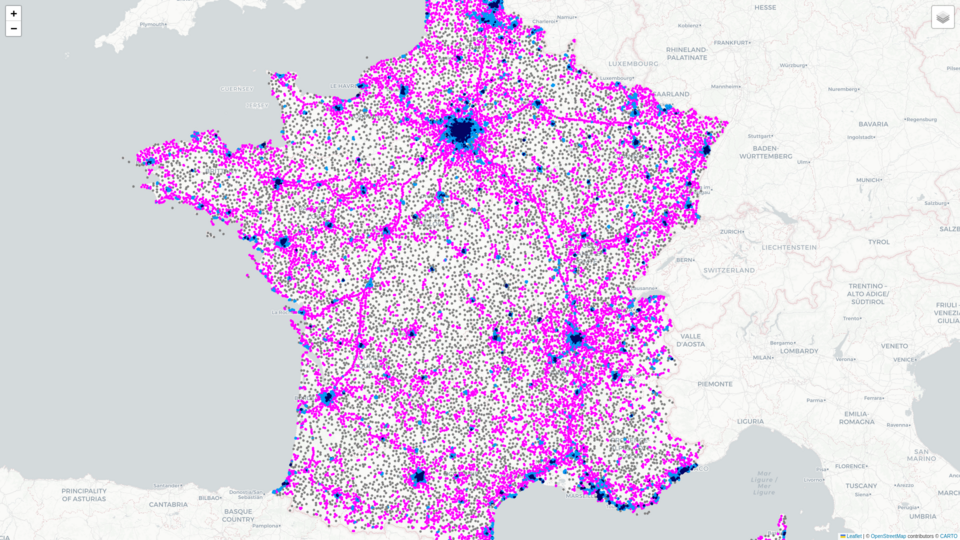
\includegraphics[height=0.6\paperheight]{images/cartes/road_detection/res.png}
        \caption{Road detection}
    \end{figure}
\end{frame}

\subsection{More details and problems}
\insertsubsectionframe

\begin{frame}{Detailed clusters detected}
    \begin{figure}
        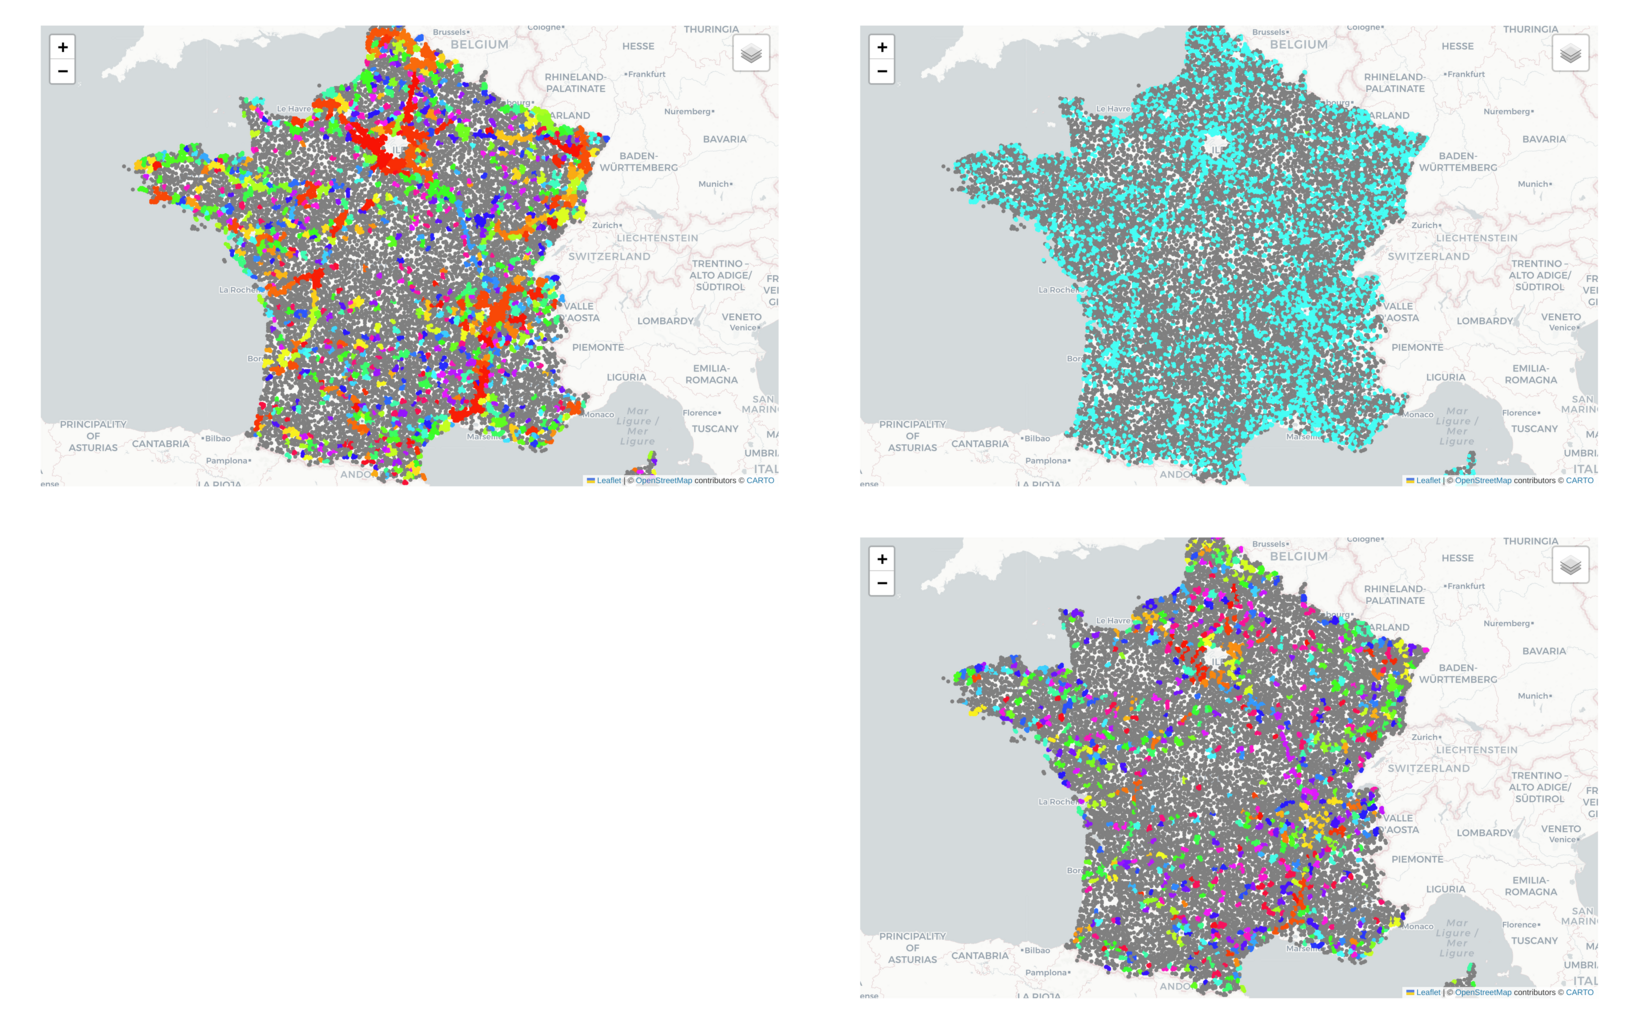
\includegraphics[height=0.6\paperheight]{images/clusters_road_detection.html.png}
        \caption{Detailed clusters detected in coutryside by each method}
    \end{figure}
\end{frame}

\begin{frame}{Problems and ideas}
    \begin{block}{Problems}
        \begin{itemize}
            \item A lot of little citys detected : not only roads ;
            \item The areas around big citys are a mess ;
            \item HDBScan has only one cluster.
        \end{itemize}
    \end{block}

    \begin{block}{Ideas}
        \begin{itemize}
            \item Refine the parameters of each method ;
            \item Use linear regressions to detect parts of roads and maybe help propagate them.
        \end{itemize}
    \end{block}
\end{frame}